%% Supplementary material for the Artemis II seismo-acoustic paper.
%% Compile:  bash compile2.sh Artemis2_paper1_supplement.tex
\documentclass[11pt]{article}
\usepackage[margin=2.2cm]{geometry}
\usepackage{graphicx}
\usepackage{amsmath}
\usepackage{siunitx}
\usepackage{booktabs}
\usepackage[font=small]{caption}
\graphicspath{{figures/}}
\renewcommand{\thefigure}{S\arabic{figure}}
\renewcommand{\thetable}{S\arabic{table}}
\setlength{\parindent}{0pt}

\title{Supplementary material for\\ ``Recording a heavy-lift rocket launch: network validation and recording requirements from Artemis~II''}
\author{Glenn Thompson, Paul Bremner, Han Byul Woo, Sue Bilek}
\date{}

\begin{document}
\maketitle

Table S1 (stations), Text S1 with Table S2, and Figures S1--S5 support the main text. They were produced by the notebooks in
\texttt{09\_artemis2\_paper} (numbers in brackets).

% Written by a notebook; edit the notebook, not this file.
\begin{table}[htbp]
  \centering
  \caption{Station locations and instrumentation, sorted by distance from SLC-39B. Gem 363, recorded under the provisional code \texttt{1R.UNK..HD1}, was 8~m from B20 according to its GPS log.}
  \label{tab:stations}
  \small
  \begin{tabular}{lrrrrp{5.2cm}}
  \toprule
  Station & Lat ($^{\circ}$) & Lon ($^{\circ}$) & Distance (km) & Azimuth ($^{\circ}$) & Instrumentation \\
  \midrule
  B14 & 28.6322 & $-$80.6158 & 0.74 & 41.4 & Trillium/Centaur, infraBSU, Gem, SmartSolo \\
  B01 & 28.6214 & $-$80.6067 & 1.53 & 115.0 & Trillium/Centaur, infraBSU, Gem, SmartSolo \\
  B03 & 28.6428 & $-$80.6236 & 1.75 & 351.0 & Trillium/Centaur, infraBSU, Gem, SmartSolo \\
  B12 & 28.6217 & $-$80.6472 & 2.65 & 256.6 & G\"{u}ralp Certimus, Gem, SmartSolo \\
  B05 & 28.6400 & $-$80.6450 & 2.76 & 300.9 & Trillium/Centaur, infraBSU \\
  B07 & 28.6072 & $-$80.5942 & 3.42 & 130.4 & G\"{u}ralp Certimus, Gem (2), SmartSolo \\
  B24 & 28.5806 & $-$80.6408 & 5.53 & 200.7 & Trillium/Centaur, infraBSU, Gem (2), SmartSolo \\
  B23 & 28.5786 & $-$80.6078 & 5.54 & 166.7 & Silicon Audio accel., Gem, SmartSolo \\
  B24RE & 28.5812 & $-$80.6433 & 5.56 & 203.3 & Gem \\
  B29 & 28.6181 & $-$80.6769 & 5.58 & 259.5 & Trillium/Centaur, infraBSU, Gem (2), SmartSolo$^{a}$ \\
  B24LT & 28.5805 & $-$80.6429 & 5.61 & 202.6 & Gem \\
  B20W & 28.5737 & $-$80.5725 & 7.58 & 141.4 & Gem, SmartSolo \\
  B20 & 28.5736 & $-$80.5722 & 7.61 & 141.3 & Trillium/Centaur, infraBSU, Chaparral M25, Gem (3), SmartSolo \\
  B20S & 28.5733 & $-$80.5722 & 7.63 & 141.5 & Gem, SmartSolo \\
  \bottomrule
  \multicolumn{6}{l}{$^{a}$ No data during the launch.}
  \end{tabular}
\end{table}
  % written by notebook 65

\section*{Text S1. Acoustic response of the 27-gallon tote enclosure}
\label{text:tote}

The protective enclosures at the USF stations, used for the \texttt{HDI} Gems, are 27-gallon
high-density polyethylene (HDPE) storage totes with snap-fit lids. To interpret the tote--free-field
comparison (main text, Section on enclosure effects) we estimate the enclosure's acoustic resonances
from simple models. The tote tapers; we use mean interior dimensions $L \approx 0.66$~m,
$W \approx 0.43$~m and $H \approx 0.375$~m, giving an air volume $V \approx 0.106$~m$^3$, and a sound
speed $c = 343$~m~s$^{-1}$. All values are order-of-magnitude estimates.

\paragraph{Air-cavity modes.} For a rigid rectangular cavity,
\begin{equation}
  f_{lmn} = \frac{c}{2}\sqrt{\left(\frac{l}{L}\right)^2 + \left(\frac{m}{W}\right)^2 + \left(\frac{n}{H}\right)^2}.
\end{equation}
The lowest modes are 260~Hz (1,0,0), 399~Hz (0,1,0), 457~Hz (0,0,1) and 476~Hz (1,1,0). No standing
waves form inside the tote below $\sim$260~Hz, above the band of the Gems (50~Hz Nyquist) and of
the analyses here; at lower frequencies the enclosed air acts as a single lumped compliance,
$C_a = V/(\rho c^2) \approx 7.5\times10^{-7}$~m$^3$~Pa$^{-1}$.

\paragraph{Lid leakage (Helmholtz resonance).} A snap-fit lid leaks. Treating the leak as a slit
$\sim$1~mm wide around the $\sim$1.5~m rim ($A \approx 15$~cm$^2$) with an effective length of
2--5~mm, the Helmholtz resonance
\begin{equation}
  f_H = \frac{c}{2\pi}\sqrt{\frac{A}{V\,L_\text{eff}}}
\end{equation}
is $\sim$90--145~Hz. End corrections lengthen $L_\text{eff}$ and lower $f_H$, and the real gap
geometry is unknown, so $f_H$ is uncertain by a large factor. Below $f_H$ the leak lets the interior
pressure follow the exterior.

\paragraph{Wall bending modes.} The tote's mass (6.1~lb, 2.77~kg) over its 1.39~m$^2$ of wall, base
and lid gives $\sim$2.0~kg~m$^{-2}$, or a wall thickness $h \approx 2.1$~mm for HDPE
($\rho = 950$~kg~m$^{-3}$); we consider $h = 2.0$--2.6~mm. For a rectangular plate of sides $a$, $b$
with bending stiffness $D = Eh^3/[12(1-\nu^2)]$ ($E \approx 1.0$~GPa, $\nu \approx 0.4$) and surface
density $\rho_s = \rho h$,
\begin{equation}
  f_{mn} = \frac{\pi}{2}\sqrt{\frac{D}{\rho_s}}\left[\left(\frac{m}{a}\right)^2 + \left(\frac{n}{b}\right)^2\right]
\end{equation}
for simply supported edges; clamped edges raise the frequencies by a factor of $\sim$1.85.
Table~S2 gives the resulting ranges, from simply supported edges with $h = 2.0$~mm to clamped edges
with $h = 2.6$~mm. Ribs, the taper, the lid rim and the logger resting on the base will shift these
values.

% Written by a notebook; edit the notebook, not this file.
\begin{table}[htbp]
  \centering
  \caption{Estimated in-vacuo bending-mode frequencies (Hz) of the tote panels.}
  \label{tab:tote_modes}
  \small
  \begin{tabular}{lrrr}
  \toprule
  Panel & (1,1) & (2,1) & (1,2) \\
  \midrule
  Base or lid ($0.66 \times 0.43$~m) & 8--19 & 15--36 & 24--58 \\
  Long wall ($0.66 \times 0.375$~m) & 10--23 & 17--40 & 31--75 \\
  Short wall ($0.43 \times 0.375$~m) & 13--31 & 29--70 & 34--83 \\
  \bottomrule
  \end{tabular}
\end{table}
  % written by notebook 65

\paragraph{Transmission at low frequency.} Even with a perfectly sealed lid, external pressure
deflects the walls and changes the interior volume. For a wall of volume compliance $C_w$, the
interior pressure is $p_\text{in}/p_\text{out} = C_w/(C_w + C_a)$. The lid alone, treated as a simply
supported plate (double sine series), has $C_w \approx 3.5\times10^{-5}$~m$^3$~Pa$^{-1}$ for the
2.1~mm wall implied by the tote's mass ($1.9$--$4.1\times10^{-5}$~m$^3$~Pa$^{-1}$ for $h = 2.6$--2.0~mm),
25--55 times $C_a$, so below the panel resonances the interior pressure follows the exterior to within
2--4\% even without leakage,
and more closely with all walls and the leak acting together. The enclosed air also stiffens the
volume-displacing panel modes, raising them above the in-vacuo values in Table~S2.

\paragraph{Totes that also house the electronics.} At the Centaur sites the infraBSU microbarometers
were installed in the same type of tote, which also served as the electronics enclosure: it contained
the digitizer, a regulator, a battery, cables and a wooden shelf. These displace part of the air,
reducing $C_a$, so the interior pressure follows the exterior even more closely at low frequencies and
the enclosed air stiffens the volume-displacing panel modes more strongly. The contents also add mass and
damping to the base and break up the (already $>$260~Hz) cavity modes. Panel resonances therefore remain
the main mechanism above $\sim$10~Hz, but their frequencies and amplitudes will differ from those of the
Gem-only totes. At B29, where an infraBSU in such a tote sits next to a free-field Gem, the infraBSU
record is 0.3--0.5~dB lower below 10~Hz and 1.6, 2.1 and 2.9~dB lower at 10--20, 20--30 and 30--40~Hz
(coherence $\geq$0.99), part of which may reflect differences between the two instrument responses. No
free-field reference exists above the Gems' 50~Hz Nyquist frequency, so the effect of these enclosures
on the infraBSU records at 50--225~Hz is unknown.

\paragraph{Expected response and comparison with the data.} The tote should therefore be acoustically
transparent at low frequencies, with panel resonances (and their associated amplification and
attenuation) beginning at $\sim$10--30~Hz and multiplying above, a possible leak resonance near
$\sim$100~Hz, and no cavity modes below $\sim$260~Hz. HDPE's internal damping (loss factor
$\sim$0.02--0.05) broadens these resonances. This agrees with the observations: the tote and free-field
records agree within 0.25~dB below 10~Hz at all three sites, and differ by $-4.2$ to $+1.2$~dB above
10~Hz in ways that vary between sites (main text, enclosure figure, panel b), as expected for resonances sensitive to lid fit,
leakage and how the tote and logger sit on the ground. Sensors recording at higher sampling rates
inside such totes, such as the infraBSUs, are exposed to the densest panel-mode region, $\sim$20--150~Hz.


\clearpage

\begin{figure}[p]
  \centering
  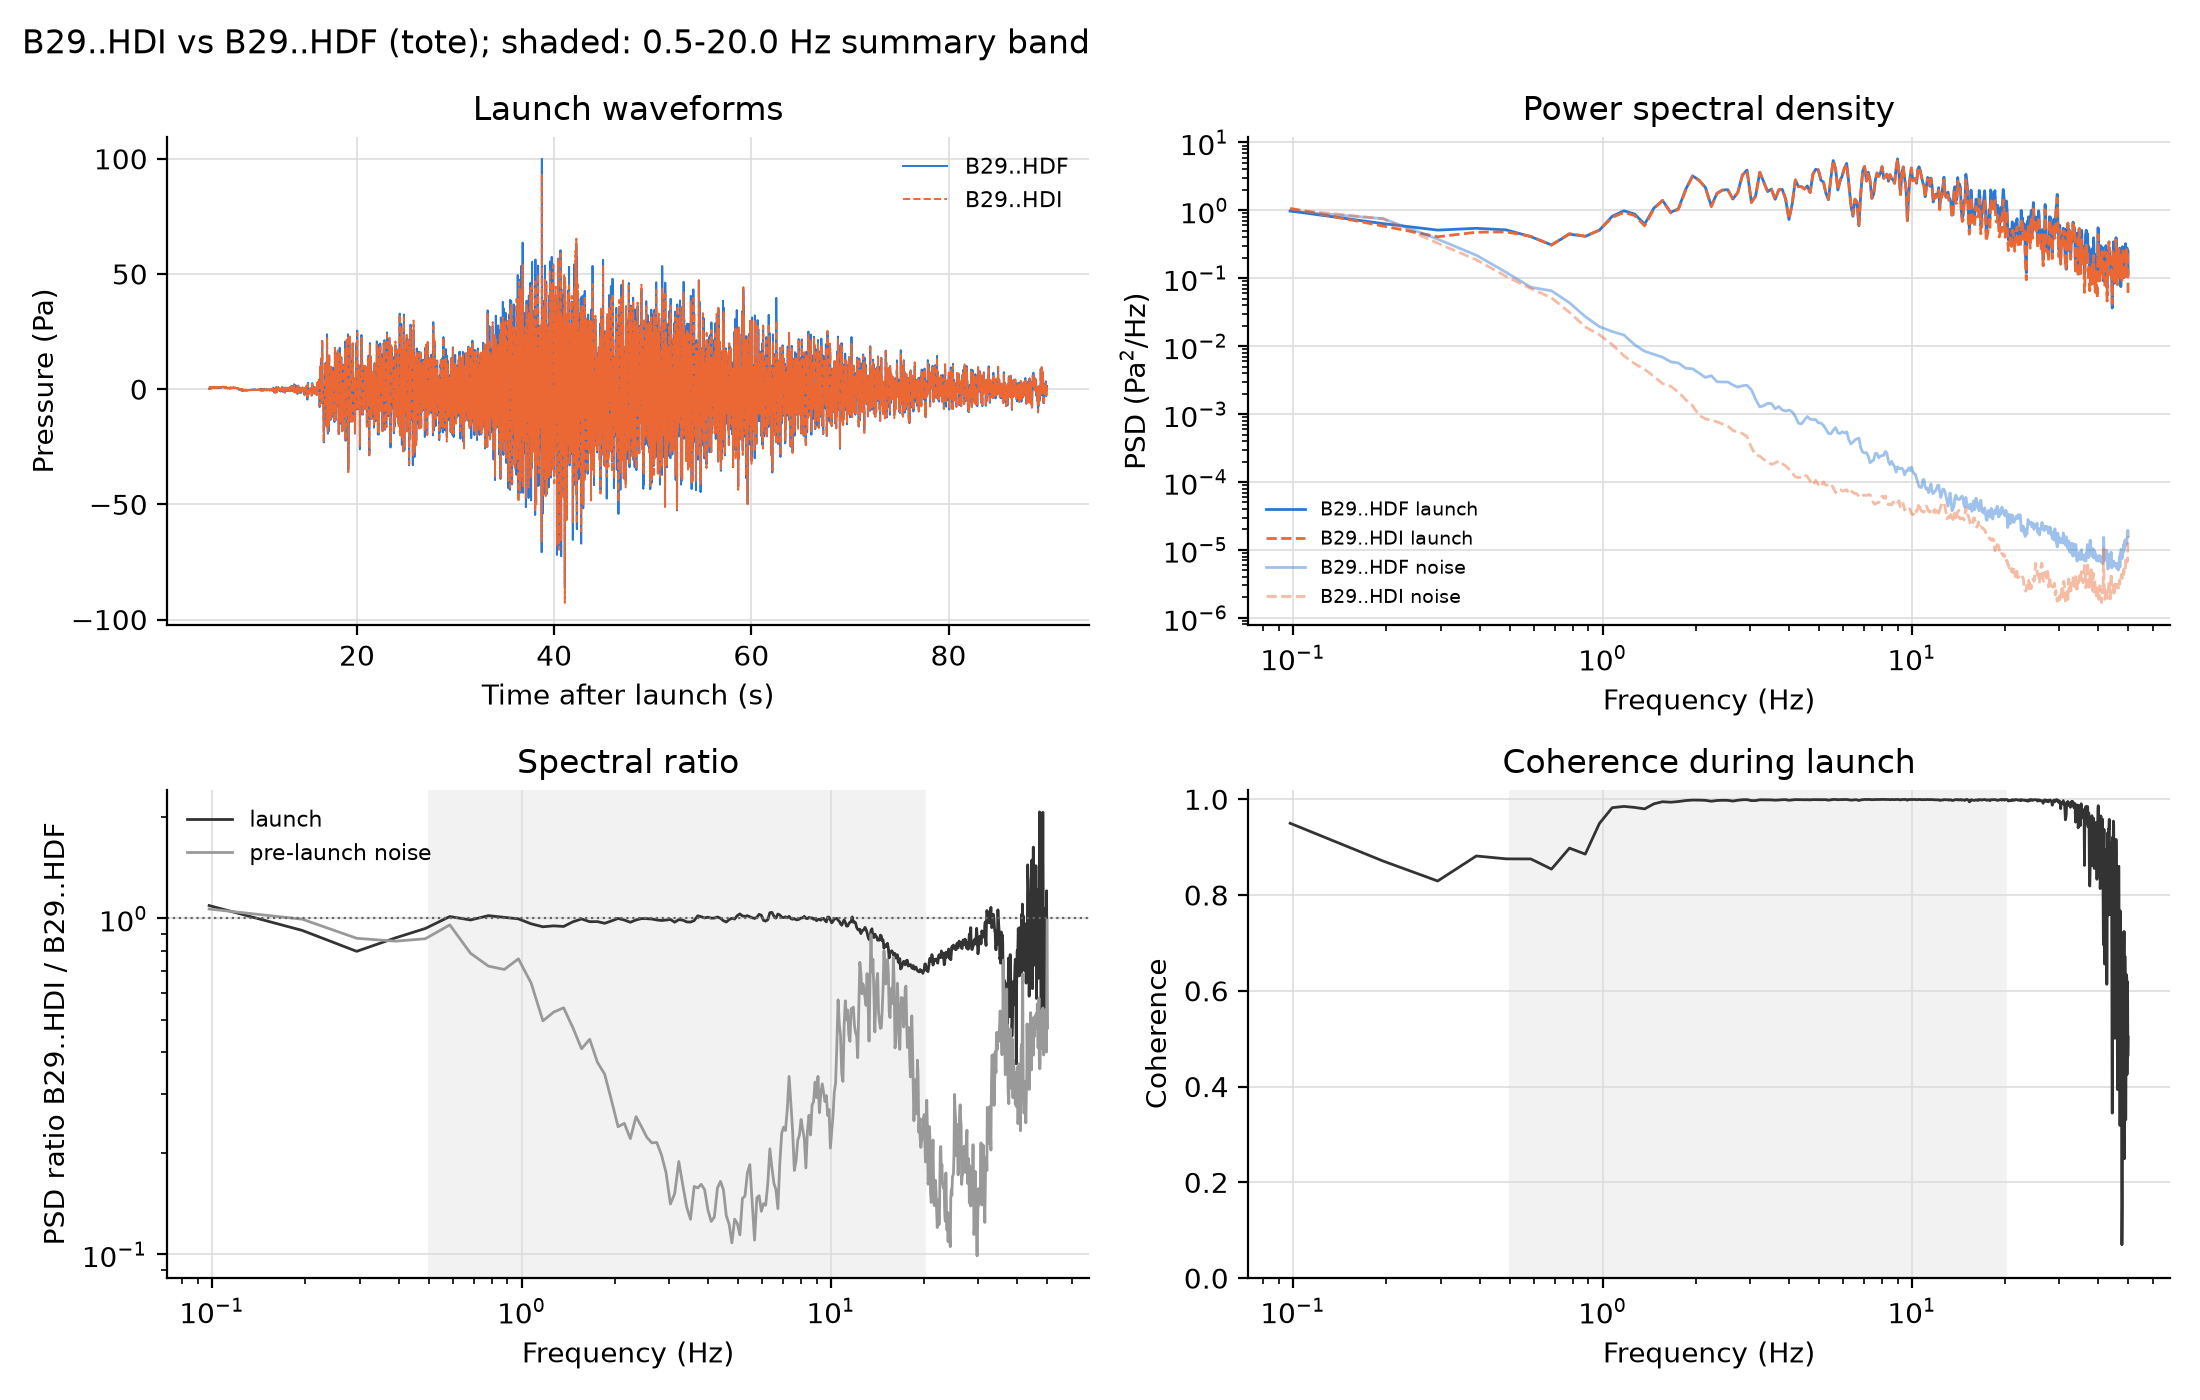
\includegraphics[width=\textwidth]{enclosure_B29__HDF_vs_B29__HDI}
  \caption{Tote (HDI) versus free-field (HDF) Gem at B29 [30]: launch
    waveforms, power spectral densities during the launch and in pre-launch
    noise, spectral ratio, and coherence during the launch. Shaded: the
    0.5--20~Hz band used for summary values.}
\end{figure}

\begin{figure}[p]
  \centering
  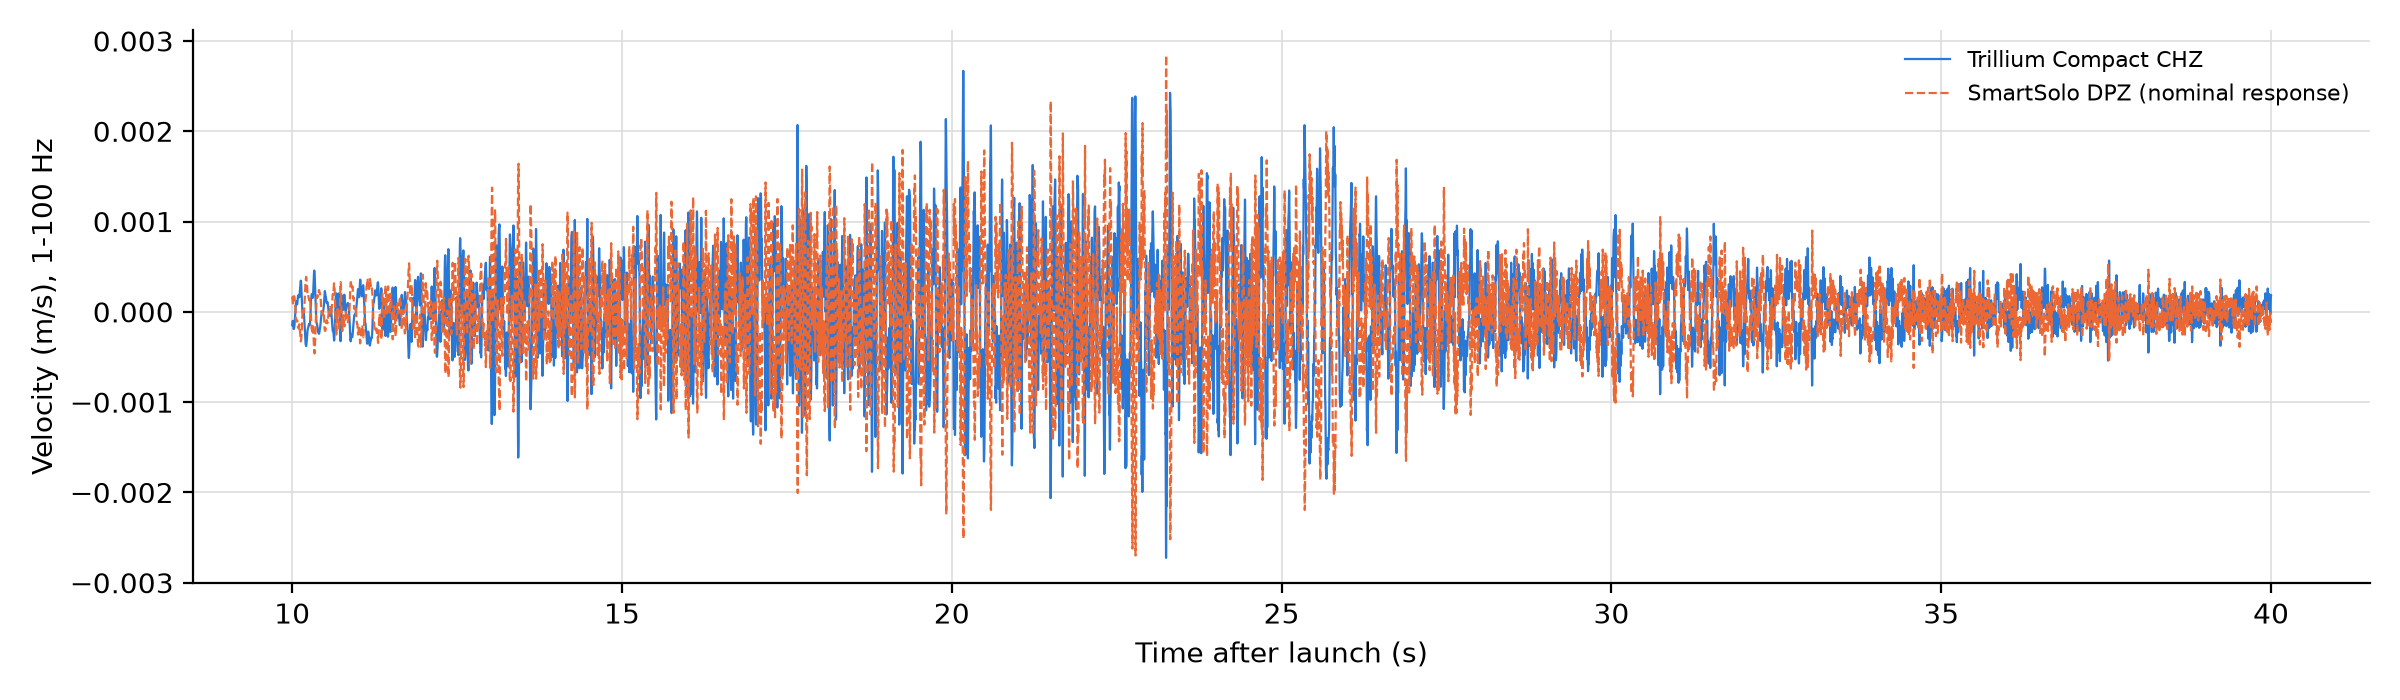
\includegraphics[width=\textwidth]{smartsolo_vs_trillium_B01_waveforms}
  \caption{Vertical velocity at B01 from the Trillium Compact (CHZ) and the
    SmartSolo node (DPZ) after removal of the nominal 5~Hz geophone response,
    1--100~Hz [45]. Peak velocities agree within 4\%. The SmartSolo trace is
    shown as recorded (reversed polarity).}
\end{figure}

\begin{figure}[p]
  \centering
  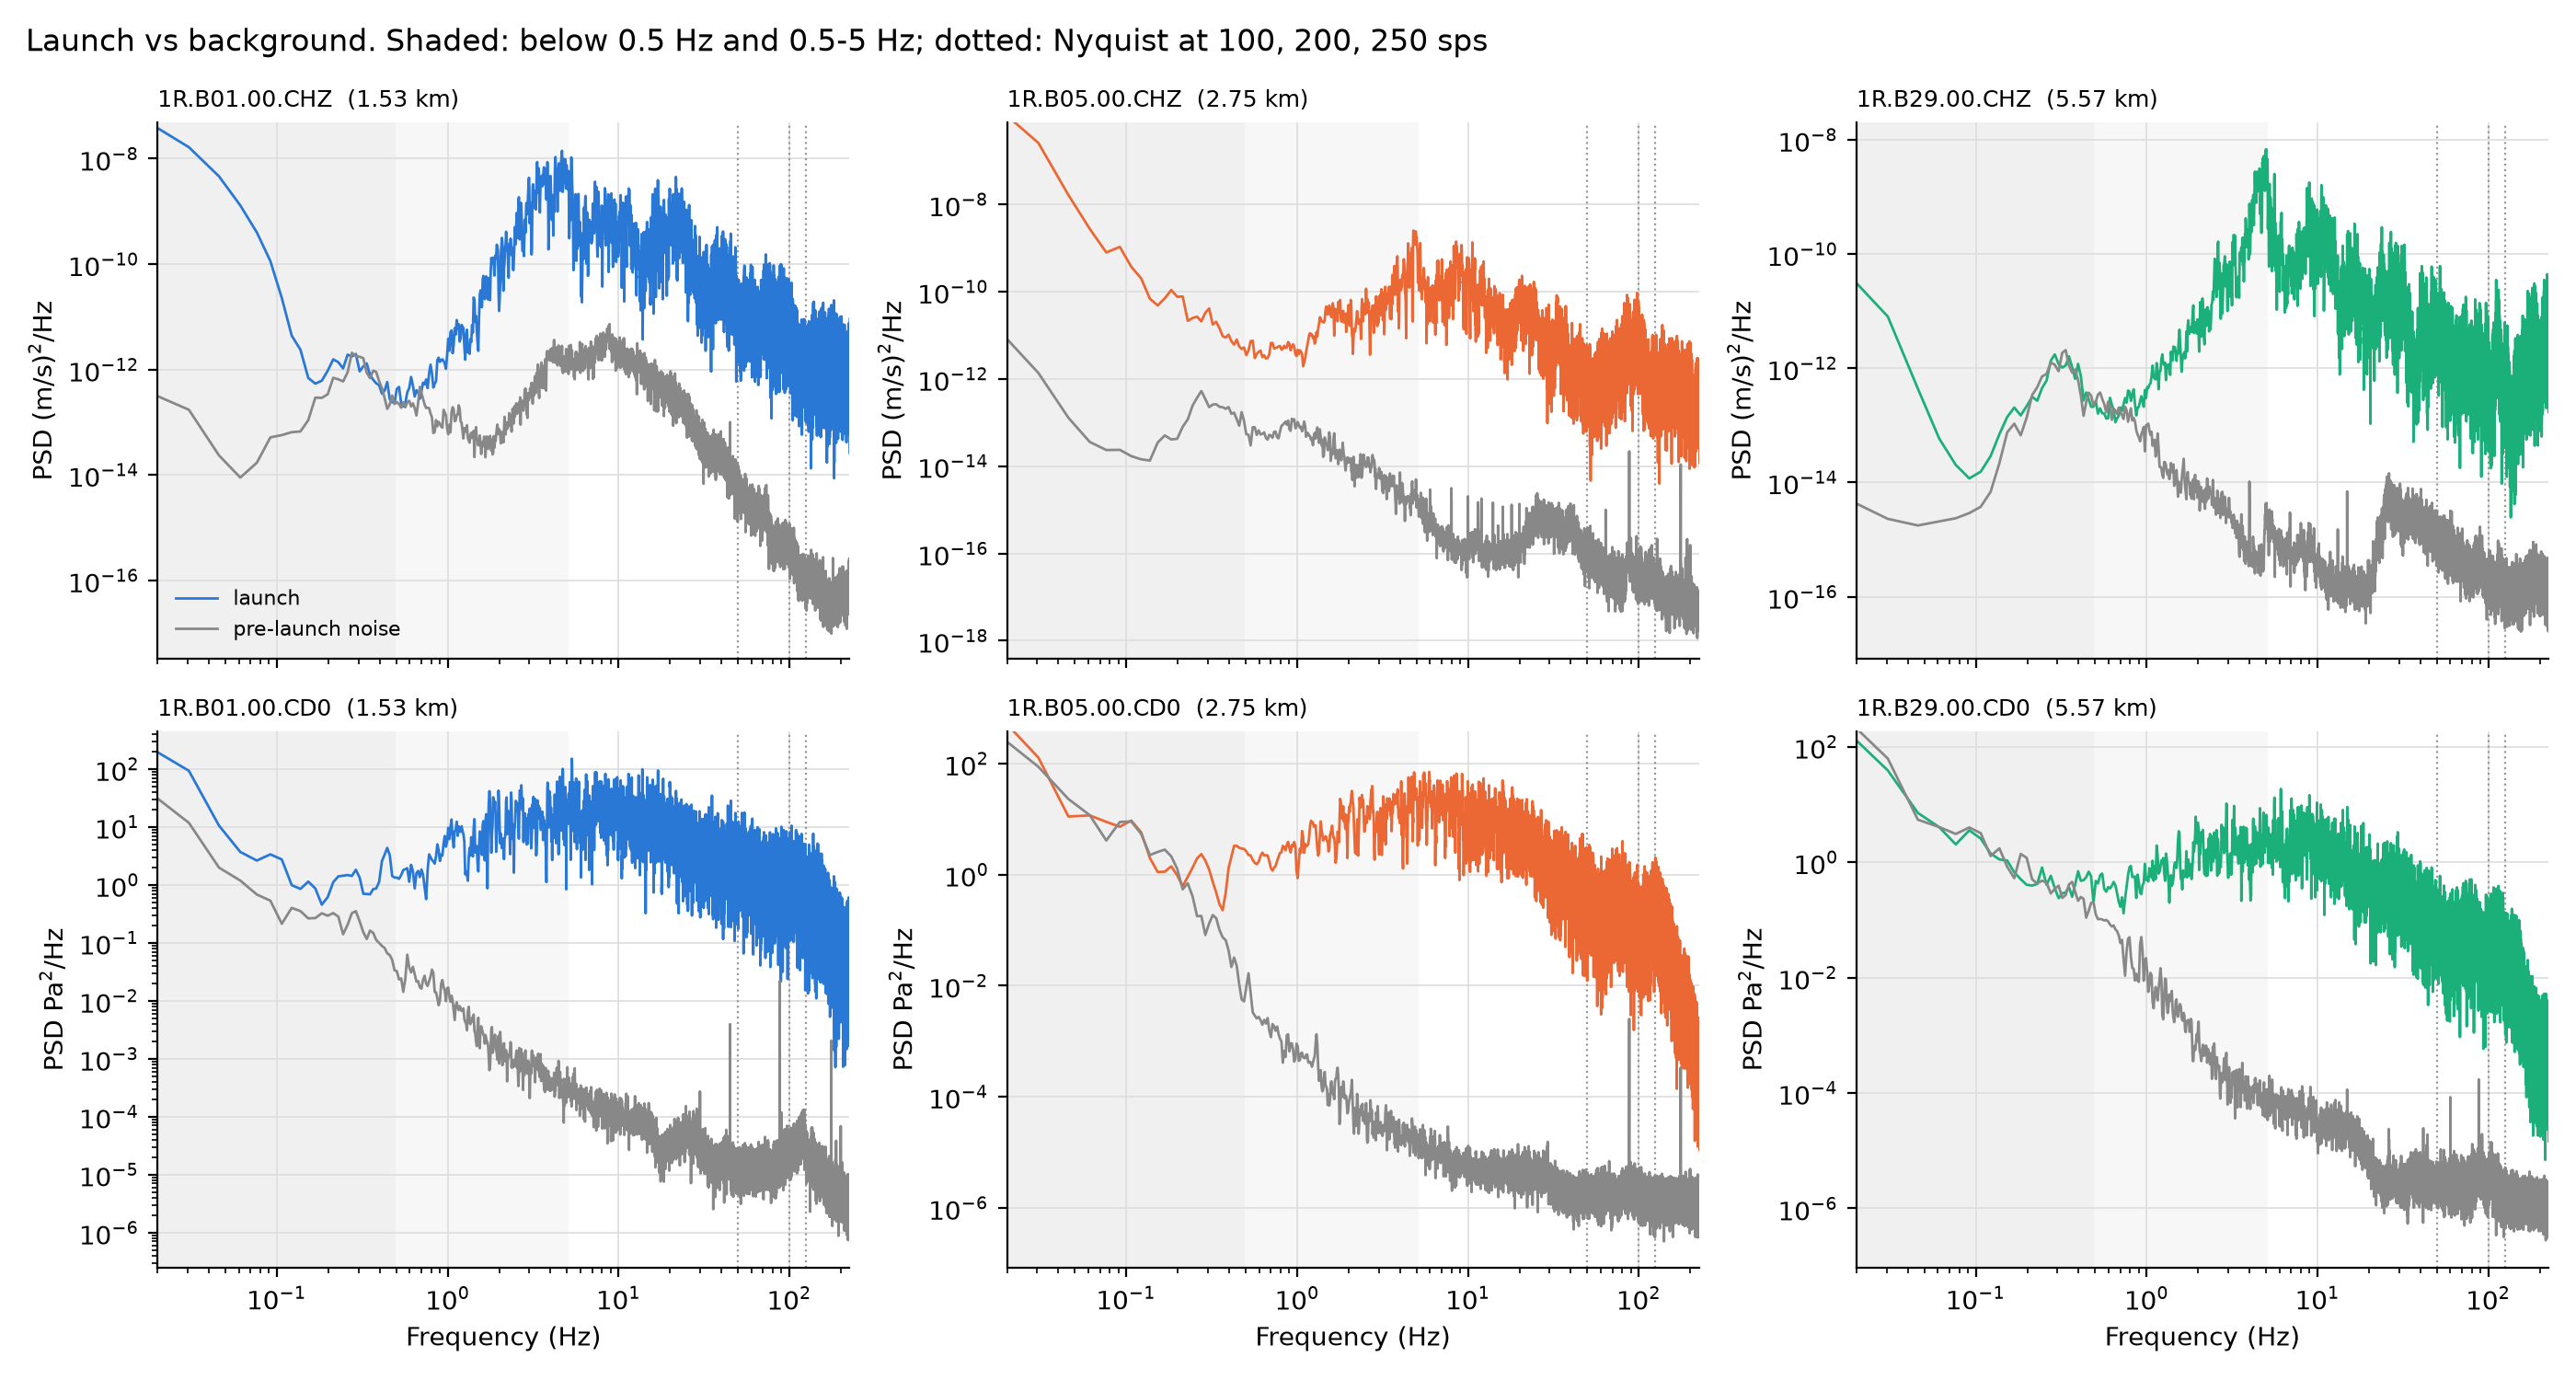
\includegraphics[width=\textwidth]{bandwidth_psd}
  \caption{Power spectral density during the launch and in pre-launch noise
    for vertical velocity (top) and pressure (bottom) at B01, B05 and B29
    [45]. Shaded: below 0.5~Hz and 0.5--5~Hz; dotted: Nyquist frequencies of
    100, 200 and 250~samples~s$^{-1}$.}
\end{figure}

\begin{figure}[p]
  \centering
  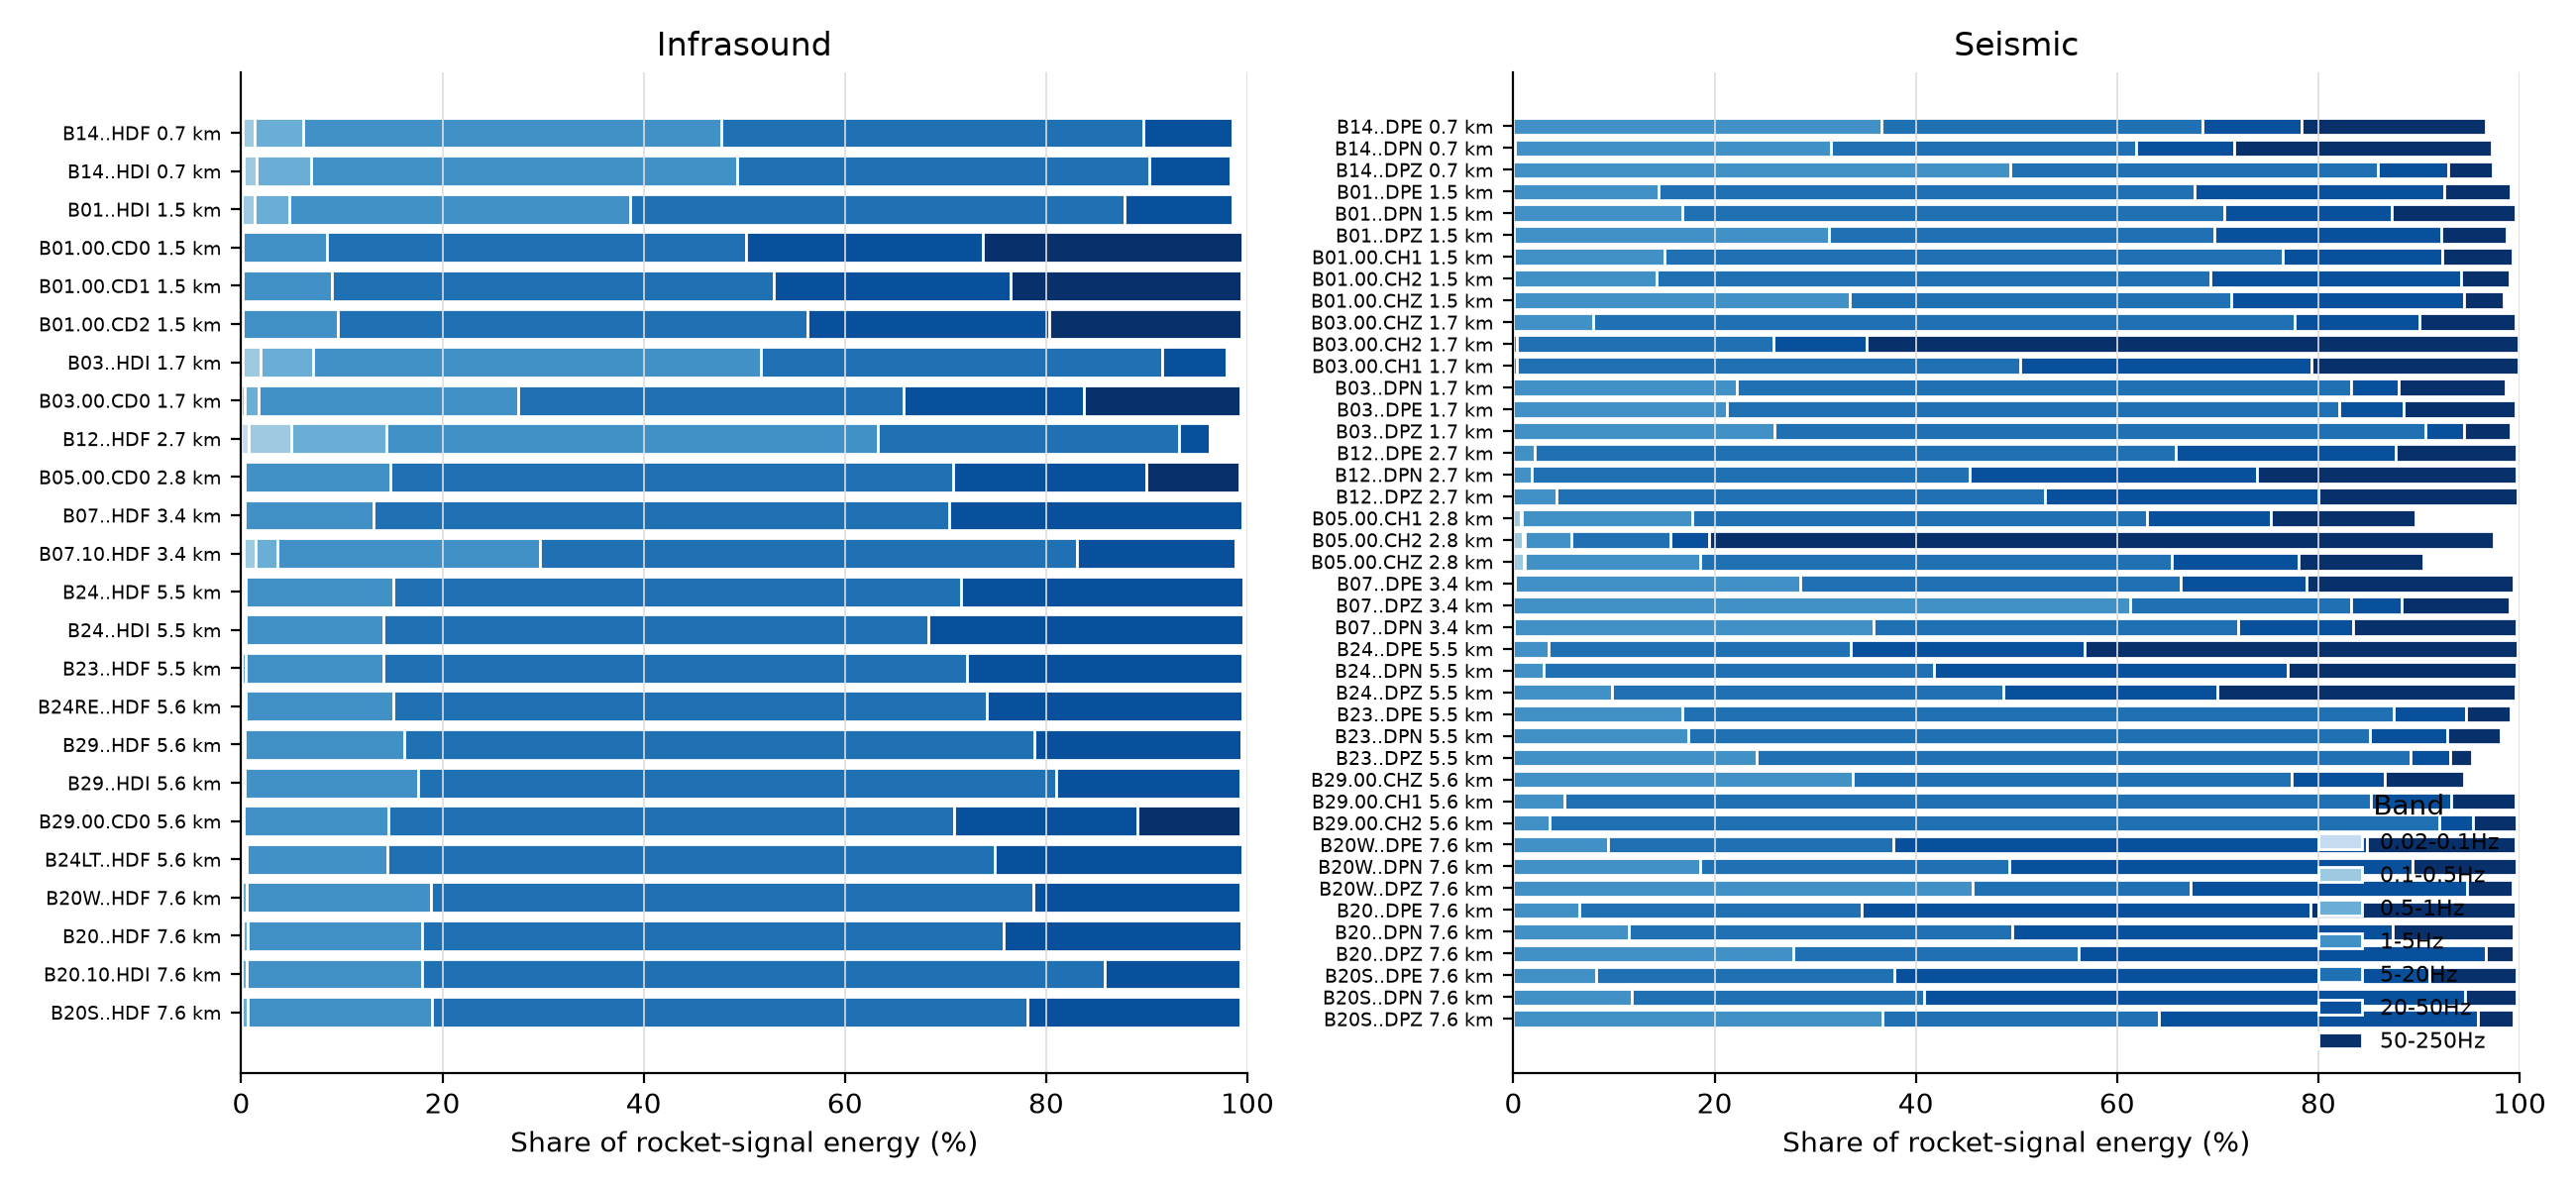
\includegraphics[width=\textwidth]{snr_band_energy}
  \caption{Share of rocket-signal energy (launch minus noise PSD) in frequency
    bands for every pressure (left) and velocity (right) channel, sorted by
    distance [42]. Gem spectra end at 45~Hz and SmartSolo spectra are
    meaningful only above 1~Hz.}
\end{figure}

\begin{figure}[p]
  \centering
  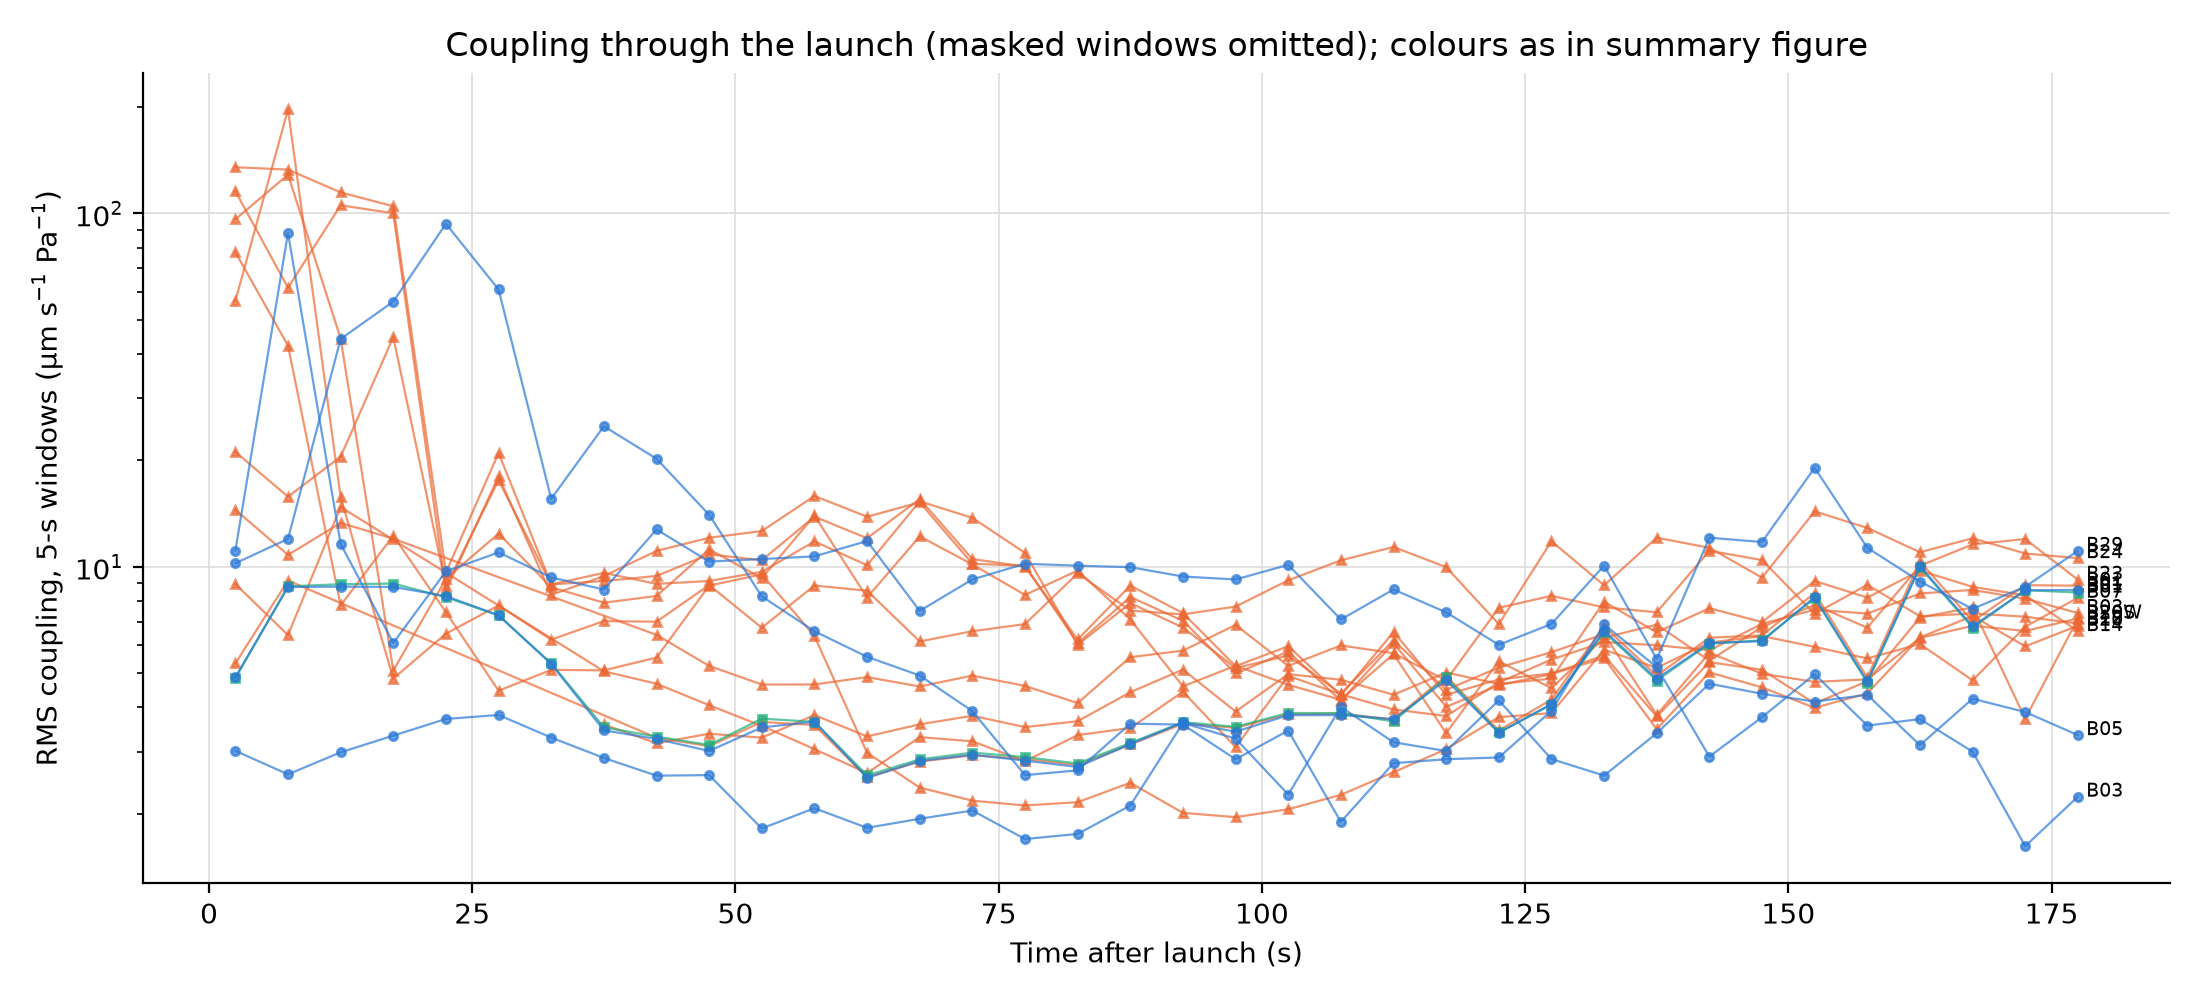
\includegraphics[width=\textwidth]{coupling_vs_time}
  \caption{RMS ratio of vertical velocity to pressure (1--40~Hz) in 5-s
    windows through the launch for each co-located pair [50]. Windows
    overlapping Gem overflow are omitted. At the distant B20 sites the ratio
    is high before the air wave arrives, because ground motion from the pad
    arrives first.}
\end{figure}


\end{document}
